%
% $Id$
%

\documentclass[10pt]{article}
\usepackage{mathptmx}
\usepackage{courier}
\usepackage[T1]{fontenc}
\usepackage{textcomp}

\usepackage{epsfig}
\usepackage{listings}

\lstdefinelanguage{MYLANG}
{morekeywords={},
sensitive=false
}

% See the dvips documentation
% Shrink figures larger than the text width to the text width
\def\epsfsize#1#2{\ifdim#1>\columnwidth\columnwidth\else#1\fi}
%\def\epsfsize#1#2{\textwidth}
\epsfverbosetrue

%\title{Declarative Implementation of Semi-dynamic Web Sites}
\title{Automated Development and Maintenance of Semi-dynamic Web Sites through Declarative Specifications}

\author{Diomidis Spinellis, Vassilios Karakoidas and Damianos Chatziadoniou\\
Department Management Science and Technology \\
Athens University of Economics and Business \\
Greece\\
email: \{dds, bkarak, damianos\}@aueb.gr}

\date{}

\begin{document}

\maketitle

\begin{abstract}
\noindent
Traditionally, the realization of Web sites involves either
static content developed using web authoring tools or dynamic
content delivered by a database driven front-end,
where the structured content is organized
in a relational schema and dynamically generated on the fly.
The limitations of statically-authored web pages are easy to discern and
for a number of applications, the use of a database
introduces a level of additional complexity that
makes the choice a part of the problem space rather than the solution space.
We introduce a different approach, which is suitable for managing 
middle-sized semi-dynamic web sites. The technological dimensions of this
approach are well-known open source technologies, such as {\sc CVS}, BibTeX 
and {\sc XML} transformation tools.
\end{abstract}

\subsection*{Keywords}
Web site implementation, Semi-dynamic web sites, {\sc XML}, make, BibTeX, {\sc XSLT}, X-Schema, {\sc HTML}.

\section{Introduction}
\label{sec:intro}
Traditionally, the realization of Web sites involves either
static content developed using web authoring tools like
Microsoft's Front Page and DreamWeaver, or dynamic
content delivered by a data-oriented front-end,
where the structured content is stored in a relational database 
and dynamically generated on the fly.
When our group faced slowstoper successive problems with both the above approaches,
we decided to adopt the task of exploring ideas for a radically different
implementation style, based on the declarative specification
of all the site's elements.

The limitations of statically-authored web pages are easy to discern.
The content is entered in an unorganized manner, and, as a result,
can be inconsistent in both structure and presentation.
While the use of cascading style sheets can help one obtain a
consistent look, their use still requires discipline.
The authored pages are however still unstructured and the resulting
site can be difficult to modify and reorganize.
Furthermore, the static authoring model often imposes a centralized
management and maintenance style;
all additions and changes have to go through a single person,
creating a bottleneck, often leading to outdated content.

Adopting a database driven approach is supposed to
solve the aforementioned problems.
Separating the source data from its (dynamically generated)
marked-up version ({\sc HTML} code) leads to a consistent
yet flexible generation of web pages.
In addition, the database's relational model imposes
its structure on the source data being stored.
Finally, a database back-end allows concurrent updates by
different users.

However, for a number of applications, the use of a database
introduces a level of additional complexity that
makes the choice a part of
the problem space rather than the solution space.
A database-driven web site requires the implementation of a
front-side interface to transform the web site's content into
{\sc HTML} code, and a back-end interface to allow stakeholders
enter, review, and update data.
The back-end client interface typically requires setting up
and maintaining appropriate access permissions.
These may need to be integrated into an organization wide single
login facility, or operated under a specific security policy.
In the second case procedures for setting up passwords,
resetting them, and revoking them need to be established and followed.
A properly running database also requires a skilled database
administrator to install it, maintain it, organize backups,
and perform modifications to the database schema.
In addition, because marked-up content is generated by a front-end
program accessing the database, both the front-end and the database
must be extremely robust, running on a $24 \times 7$ schedule.
The front-end, being an executable program working on
untrusted data (the web page requests) can become the target of
malicious attacks,
and must therefore be inspected and audited to ensure its robustness.
To minimize the risk of an attack against the database
(that would jeopardize the organization's data)
the database server has to be installed on a machine separate
from the web server, behind a (properly configured) firewall.
Finally, the extraction of content from a database often
induces the web site's designers and stakeholders to adopt a
query-style interface.
Such an interface is typically less usable than browsable web pages,
and the served content is often ignored by search engines,
leading to reduced visibility
of the (meticulously structured) content \cite{DEEP_WEB} \cite{JP04}.
All in all, a database-driven approach appears to be suitable
only for those with ample resources to justify the full
development and appropriate maintenance of a sophisticated infrastructure.

Having faced the problems we described above within our organisation we reasoned that
a fresh approach was needed for this problem and tackling them to 
set up a project for finding it.
The ad-hoc authoring tool--based approach was abandoned,
because it led to an inconsistent look and stale content,
while the maintenance of a subsequent database-driven
design approach was proving intractable for the resources that
our group could afford.
Our goal was to experiment with a different approach,
proving its suitability for managing middle-sized semi-dynamic
web sites.

\section{Requirements}
\label{sec:req}

\begin{figure}
\begin{center}
\leavevmode
\epsfbox{Diag.eps}
\end{center}
\caption{
\label{fig:diag}
Overview of data element relationships.}
\end{figure}

The functional requirements for our center's site were
simple, but not trivial, and had already been satisfied
twice in two different forms.
The site's pages should represent the content and the relationships
we illustrate in Figure \ref{fig:diag}.
The center consists of multiple research groups.
Members of our center and our research projects are
associated with the center as a whole, and, typically, also
with one or more research groups.
Publications, such as journal articles and books,
are also associated with the center, individual members (the authors),
projects that funded the corresponding work,
and groups that performed the work.
Note that members, publications, and projects associated
with one or more groups are aggregated and are typically associated
again with the research center as a whole.
For the sake of simplicity,
we have omitted from our description and the diagram
a number of additional relationships,
such as the member directing a group or managing a project.
As an example of the type of content we were looking for,
the research center, 
each member, group, or project should have a web page with a list
of the corresponding publications;
the research center and each group should have pages listing
their projects and members. 
In order to add in our web site data that is not part of the aforementioned categories,
each group can have additional pages of unstructured center's content.
Finally, each member of our groups could be performing a presentation in our group weekly seminar.

As we hinted in the previous paragraph, the problem with
the previous implementations was not the creation of the site
satisfying the functional specifications,
but the lack of a number of important non-functional requirements.
Before embarking on our third attempt,
we articulated those non-functional requirements
we thought important, to ensure that our third attempt would produce
a result with a longer life span.
The following is a list of the non-functional properties
we deemed important enough to guide our design.

\begin{description}
\item[Openness] The tools used in the realization of the web site
should be available as open source, or supported by multiple vendors.
We wanted to avoid becoming tied with a particular proprietary
tool.
We reasoned that openness would mitigate two risks:
(1) finding a maintainer trained to use a particular proprietary tool,
and (2) obtaining resources for upgrading and maintaining the tool.

\item[Observability]
The semantic distance between
the specification of an element and its implementation 
should be minimal \cite{SG97}.
The site's look and content should be maintainable
using standard tools and techniques.
If possible, the site's maintainer should not be required to
learn a scripting language like {\sc PHP}, or {\sc Perl}, or
a framework like {\sc J2EE} or {\sc .NET}.
An approach based on declarative specifications \cite{FFLS00} and
domain-specific languages \cite{DKV00} \cite{Spi00b} would allow end-users, or members
close to end-users be involved in maintaining the site,
without risking the bottleneck of going through
multiple intermediaries.

\item[Robustness] The web site should not depend on
any external programs other than the web server for serving
its content.
Users updating the data, should be able to author, validate and 
review their changes without requiring network connectivity.
This would allow them to work productively over dial-up connections
or while on the road. In addition, all the editing users should be able 
to work on a platform of their choice ({\sc UNIX}, {\sc WINDOWS} and {\sc MACINTOSH}) 
with only a simple text editor.
Minimizing the dependencies on additional servers (such as a
database or an application server) and on the network
should result in a more robust and easier to maintain system.   

\item[Parsimony] The implementation effort for
implementing the system should be minimal.
This would minimize errors and maintenance costs.
We reasoned we could satisfy this requirement by
using existing tools, if their choice satisfied the
other non-functional properties.
\end{description} 

\section{Design Process}

\subsection{Conceptual Framework}

The system's conceptual framework is illustrated in Figure \ref{fig:conc-model}.

\begin{figure}[h!]
\begin{center}
\includegraphics[scale=0.6]{conc-model}
\end{center}
\caption{Conceptual design of our system}
\label{fig:conc-model}
\end{figure}

The main concept in our system is the \textit{Organisation}. Each \textit{Organisation} has 
information that interests \textit{Content Consumers}. They 
can access the organisation's \textit{Public Data}.
These are typically information regarding the \textit{Organisation}.
It has also \textit{Content Developers} 
who are usually its members. \textit{Content Developers} update the 
\textit{Public Data} for the \textit{organisation}.

\textit{Content Administrators} are supporting the \textit{Content Developers} 
(mostly troubleshooting and account management)
and inspecting the submitted \textit{Public Data}.

\subsection{Motivation and Design Paradigm}

Our main guiding principle was to create a continuous multi-person 
development activity.
Live web sites continuously evolve;
adopting the content authoring paradigm implied
by the first approach was a mistake.
Empirical evidence supports this observation.
Figure \ref{fig:rankyear} illustrates the changes
in usability rankings given to 21 Greek government department
web sites between the years 2002 and 2003 \cite{G03}.
The X shape in the rank changes between the one year and the next
is, we believe, the result of statically authored web pages
degrading to a point of irrelevance, and then being overhauled
from scratch. The change of ranking can be explained as decay of the web site when dropping,
and re-engineering when rising.

A database-driven approach also hinders evolution.
Changes to the content's presentation require the modification
and installation of the front end page generator;
not a typical lightweight operation.
Changes to the data schema are even more intrusive
requiring a synchronized modification of the data,
the front end, and the back end.

\label{sec:design}
\begin{figure}[h!]
\begin{center}
\leavevmode
\def\epsfsize#1#2{\epsfxsize}
\epsfysize.8\vsize
\epsfbox{rankyear.eps}
\end{center}
\caption{Yearly changes in web site rankings}
\label{fig:rankyear}
\end{figure}

Continuous multi-person development projects are quite
common in software development.
Numerous developers contribute and coordinate their work
through a version control system, like {\sc CVS} that
maintains a master repository of the source code.
Concepts like the daily build \cite{CS95b} or the
current and stable branches as practiced by
numerous open source projects allow the maintenance
of a known-good product.
What we needed for our approach were appropriate
declarative language-based formalisms for expressing our data,
its transformation into {\sc HTML} pages, and the
generation process. We were clear that we wouldn't support the content in a makefile \cite{OTT91}.

\subsection{Processes}

\begin{figure}[h!]
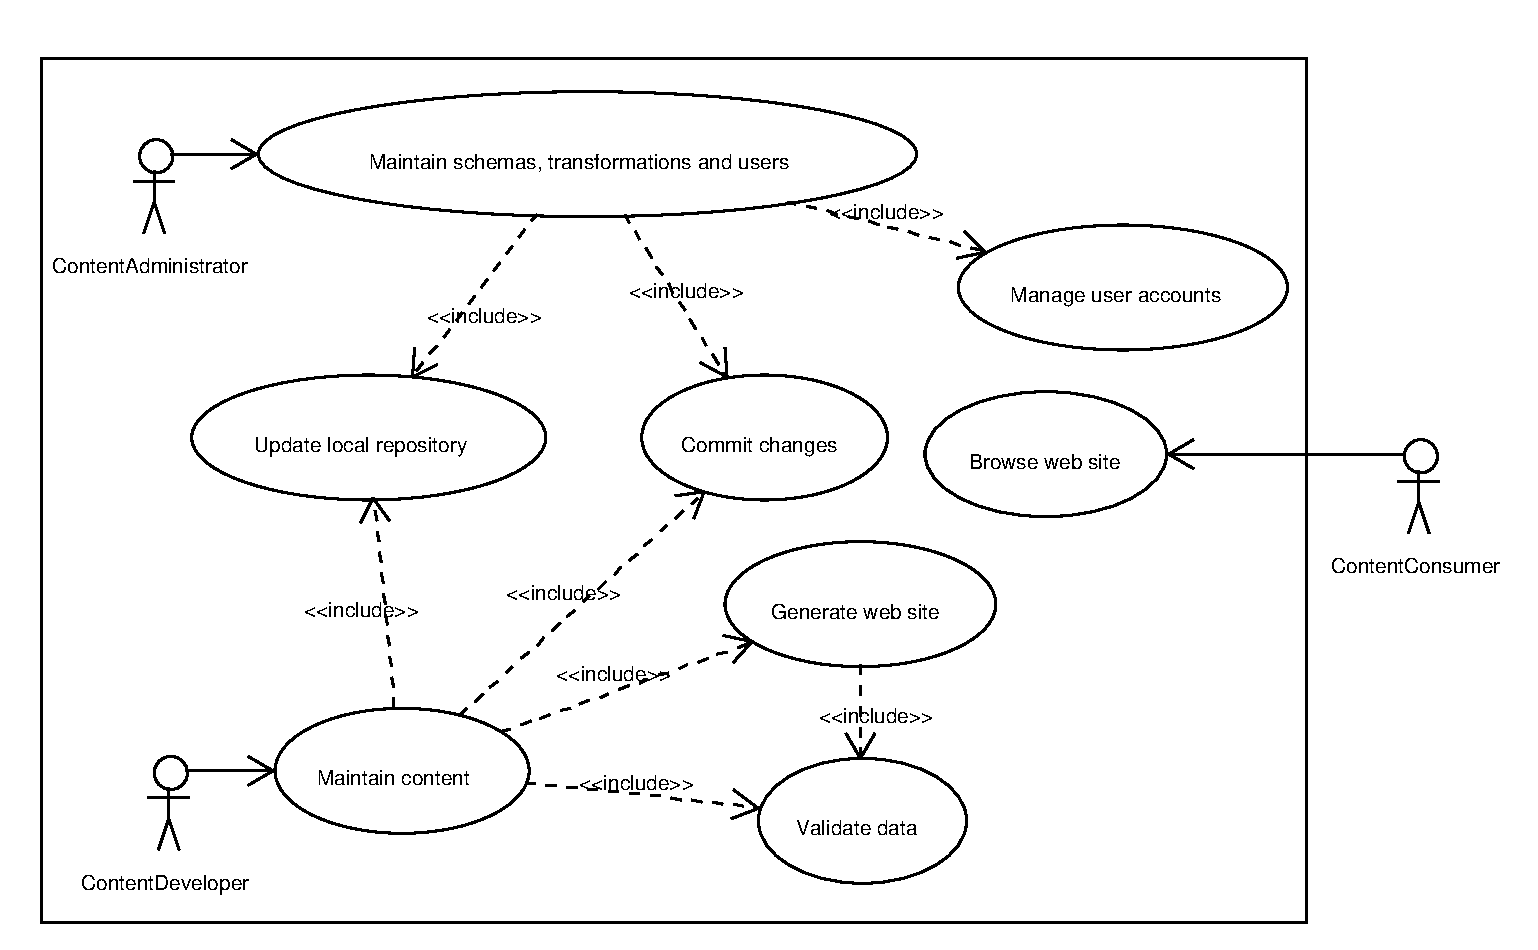
\includegraphics[scale=0.5]{use-case-diagram}
\caption{UML Use Case Diagram of the System}
\label{fig:use-case-diagram}
\end{figure}

Figure \ref{fig:use-case-diagram} shows a {\sc UML} \cite{UML} use case diagram of our system. 
We have three actors (roles) interacting with the system:

\begin{description}
\item[ContentDeveloper] A content developer is responsible for uploading data in the system. 
In our case is typically a person for each research group. He can upload data files and 
import new bibliography entries.

\item[ContentAdministrator] The content administrator is responsible for the maintenance 
and the further extension of the system. He corrects problems with the data, develops 
new features or corrects existing ones in the transformation scripts.

\item[ContentConsumer] The content consumers are typically outside of our system
and have access only in the generated web site.
\end{description}

The use cases that comprise our system are:

\begin{figure}
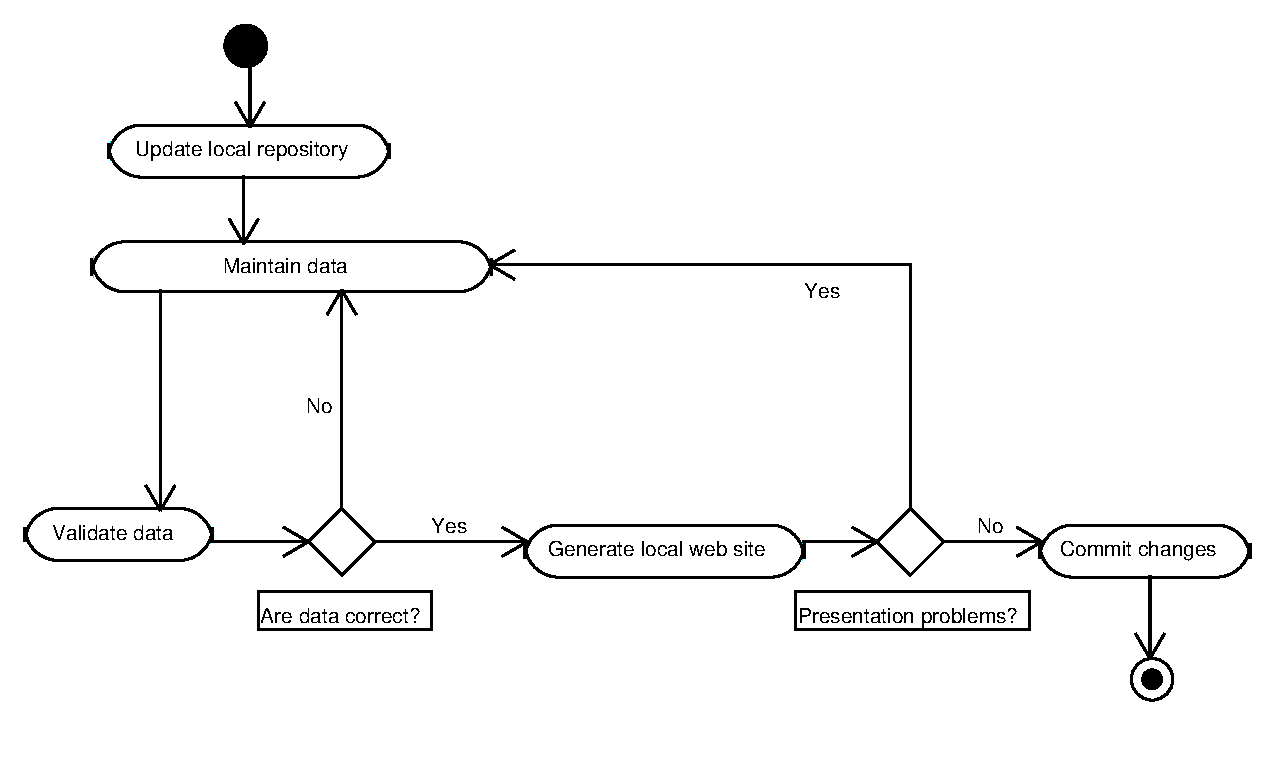
\includegraphics[scale=0.5]{maintain-content-activity}
\caption{UML activity diagram for Maintain Content}
\label{fig:maintain-content-diagram}
\end{figure}

\begin{description}
\item[Maintain schemas, transformations and users] This use case describes the 
maintenance and development procedures of the system. Each Content Developer can
update the Data schemas, the transformation scripts in order to correct errors 
or add new features.

\item[Update local repository] Each user in the system must update the local 
repository each time he uses the system. To do so, they must execute a  update 
repository command. If there is a conflict, the users must correct the problem 
and rerun the update command.

\item[Commit changes] Content developers and Content administrators must commit 
the changes from their local repository to the {\sc CVS} repository in the web site server.

\item[Maintain content] This is the overall use case that allows Content 
Developers to maintain the content of the web site. 
Content consists of  group, member, project and seminar data or bibliography 
collection entries.

\item[Generate web site] Content administrators and developers can generate the 
web site locally for preview. This procedure is 
performed with the execution of a make file command. Upon completion, 
the user can review the newly integrated content and inspect 
for possible presentation problems.

\item[Validate data] Content developers can validate the data in the local 
repository before the final commit. For the validation procedure
the system use the appropriate data schemas.

\item[Manage user accounts] Content Administrators perform user management in the 
system. User management consists mainly of two main processes: 
(1) Authentication , (2) Ownership \& Policy

\item[Browse web site] This one describes the we site browsing process. Only 
Content Consumer can access the generated {\sc HTML} pages.

\end{description} 

In figure \ref{fig:maintain-content-diagram} we show the activity diagram of the 
most complex use case in the system. The Content Developer first updates the 
local repository and then begins the initiation of data maintenance by adding, 
removing or modifying data files and bibliography entries. Upon completion data 
validation must be performed before the commit to the data repository. If data 
are valid, then local web site generation must be performed to correct possible 
presentation problems. After that, the data are ready to be submitted to the main 
data repository. After the update of the data repository the process terminates.

\section{Implementation}

\subsection{Key Technologies}

Once the design was finalized,
implementation proved to be an almost hollow activity,
since it did not involve almost anything of what
is typically described as coding.

The first step involved selecting and setting up the
appropriate tools. In order to meet the requirements we set in section \ref{sec:req}, 
we decided to use open and popular
technologies as key elements of our system.
We adopted the concurrent versions system
({\sc CVS}) \cite{BF01} \cite{CVS} to coordinate the distribution
and update of all the system's components.
Authentication for managing content was handled by the
Unix group membership mechanism of the host where the
{\sc CVS} repository was installed.
We also used
{\sc BibTeX} \cite{Pa88} \cite{Lam94} and {\sc bib2xhtml} \cite{BibXHMTL} for transforming the publications
into {\sc HTML} and
xmlstarlet \cite{Gru04} for validating and transforming
all other {\sc XML}-based data \cite{W3C_XML}.
For data transformations we 
implemented a system based on XSLT \cite{W3C_XSLT}, a language for transforming XML documents.
Finally, {\sc GNU} make \cite{gnu_make} and a couple of shell script
constructs were used for handling the project's makefile.
The complete setup including all tools proved to be portable
between Unix and Microsoft Windows, with team members working
on machines running different versions of {\sc Windows}, {\sc GNU/Linux},
and {\sc FreeBSD}.

\subsection{System Development}

The next step was a series of iterations where we
modeled the data's schema on representative {\sc XML}
files. Concurrently we implemented the validation {\sc DTD/XSDs}
and the transformation {\sc XSLTs}. First we developed the {\sc DTDs}
for the data validation, later on we decided to move in {\sc XSD} schemas in order to
further data validation to our system.
The version control system was already proving its value
at this point
for coordinating the work between the two paper's authors.
Because many page elements, like a project's description,
could contain content more elaborate than plain text,
we used W3C's modular {\sc XHTML} specification for
importing existing elements in our {\sc DTD/XSDs}.
This helped us keep our schema description simple,
but the corresponding schema expressive.

The automated validation and generation of content was
expressed as makefile rules.
The individual files {\sc XML} files are merged in a
single {\sc XML} file for cross validating identifier
reference attributes ({\sc IDREFs}).
The same file is used to extract the identifiers of
all projects, members, and groups into makefile
variables.
A simple loop then generates the {\sc HTML} files
corresponding to each of the above elements.
Each project, member, group etc. refer to the relevant {\sc XML IDs}.
Upon generation process of the {\sc HTML} pages, links are created that
connect relevant pages e.g. each member connect with his publications, 
which are two different independently generated {\sc HTML} pages.

The {\sc HTML} content is by default generated on the
local machine, where its maintainer can verify it.
After the new content is validated and verified,
the maintainer can commit the change to the central {\sc CVS} repository. 
A separate makefile rule can then be used,
to execute an update command on the
host serving the content to the web.
The command retrieves the updates from the {\sc CVS}
repository and regenerates the pages on the web-server's
file area.
All components of our system are under version control,
all pages are automatically tagged with identifiers
denoting their source, helping the traceability of changes.
All exchanges between the developers' machines and the
{\sc CVS} and web host are performed using the secure
shell ({\sc SSH}) as transport protocol guaranteeing the data's integrity
and confidentiality.

\begin{figure}
\lstset{language=MYLANG,basicstyle=\ttfamily}
{\begin{lstlisting}
<xs:schema xmlns:xs="http://www.w3.org/2001/XMLSchema">
 <xs:element name="seminar">
  <xs:complexType>
   <xs:sequence>
    <xs:element name="sem_date">
     <xs:simpleType>
      <xs:restriction base="xs:string">
       <xs:pattern value="[0-9]{8}" />
      </xs:restriction>
     </xs:simpleType>
    </xs:element>
    <xs:element name="sem_time" type="xs:string" />
    <xs:element name="sem_title" type="xs:string" />
    <xs:element name="sem_room" type="xs:string" />
    <xs:element name="sem_url" type="xs:string" minOccurs="0" />
    <xs:element name="sem_duration" type="xs:string" />
   </xs:sequence>
   <xs:attribute name="by" type="xs:string" />
  </xs:complexType>
 </xs:element>
</xs:schema>
\end{lstlisting}}
\caption{Seminars X-Schema file}
\label{fig:project-dtd}
\end{figure}

\begin{figure}
\lstset{language=MYLANG,basicstyle=\ttfamily}
{\begin{lstlisting}
<?xml version="1.0"?>
<seminar by="m_bkarak">
 <sem_date>20040314</sem_date>
 <sem_time>19:00</sem_time>
 <sem_title>Regular Expressions</sem_title>
 <sem_room>906</sem_room>
 <sem_url>http://www.eltrun.gr/seminar/presentations.ppt</sem_url>
 <sem_duration>3 hrs</sem_duration>
</seminar>
\end{lstlisting}}
\caption{A typical seminar XML file}
\label{fig:project-xml}
\end{figure}

\begin{figure}
\lstset{language=MYLANG,basicstyle=\ttfamily}
{\begin{lstlisting}
<xsl:template match="seminar" mode="full">
 <h3><xsl:value-of select="sem_title" /></h3>
  <xsl:element name="a">
  <xsl:attribute name="name">
   <xsl:value-of select="sem_date" />
  </xsl:attribute>
</xsl:element>
 Presenter: <xsl:apply-templates 
 	     select="/eltrun/member_list/member [@id=current()/@by]" 
	     mode="simple-ref" /><br />
 Date: <xsl:call-template name="date">
	<xsl:with-param name="date" select="sem_date" />
       </xsl:call-template> <br />
 Time: <xsl:value-of select="sem_time" /><br />
 Duration: <xsl:value-of select="sem_duration" /><br />
 Location: <xsl:value-of select="sem_room" /><br /><br />
 <xsl:element name="a">
  <xsl:attribute name="href">
   <xsl:value-of select="sem_url"/>
  </xsl:attribute>
  Download the presentation
 </xsl:element>
</xsl:template>
\end{lstlisting}}
\caption{The XSLT transformation file for seminars}
\label{fig:project-xslt}
\end{figure}

\begin{figure}
\lstset{language=MYLANG,basicstyle=\ttfamily}
{\begin{lstlisting}
<tbody valign="top">
<tr>
<td align="left" width="82%">
<h2>Eltrun Seminars</h2>
<a href="index.html#20040314">14 March 2004 - Regular Expressions</a>
<br><br><br>
<h3>Regular Expressions</h3>
<a name="20040314"></a>
Presenter: 
<a href="../members/m_bkarak.html">
Mr. Vassilios Karakoidas
</a><br>
Date: 14 March 2004<br>
Time: 19:00<br>
Duration: 3 hrs<br>
Location: 906<br><br>
<a href="http://www.eltrun.gr/seminar/presentations.ppt">
Download the presentation
</a>
\end{lstlisting}}
\caption{A generated HTML seminar file}
\label{fig:project-html}
\end{figure}

You can see representative samples of a project's
{\sc XSD} schema description in figure \ref{fig:project-dtd},
{\sc XML} data in figure \ref{fig:project-xml},
XSLT transformation in figure \ref{fig:project-xslt},
and {\sc HTML} result in figure \ref{fig:project-html}.

\begin{figure}
\includegraphics[scale=0.8]{distro.eps}
\caption{Directory structure of local repository}
\label{fig:eltrun-web-distro}
\end{figure}

Our system has a distribution that works in both {\sc windows} and 
{\sc UNIX} Environments (both Linux and Free BSD). The directory structure of a typical 
local repository is depicted in Figure \ref{fig:eltrun-web-distro}.
Most of our users are working in {\sc windows} environments and as 
a result we decided to upload a {\sc windows} version of the needed tools 
in the main repository under the directory \textit{bin}. The installation procedure is very simple,
and the bootstrap tools that requires are only {\sc CVS} for 
the initial check out and a ssh client. The needed keys 
for the secure shell session are provided once in each user by the Content Administrator. 
A full version of the system now demands 8 megabytes of space 
in local machine, plus some extra for the local content store and generation.

\begin{figure}
\includegraphics[scale=0.6]{dep-graph.eps}
\caption{Dependency graph of web site}
\label{fig:eltrun-web-m-dds-snapshot}
\end{figure}

In Figure \ref{fig:eltrun-web-m-dds-snapshot} we illustrate a web graph \cite{KRRSTU00} 
that shows references between the {\sc HTML} pages.
The above figure shows the references  of a member ("m\_dds" is the ID for 
Diomidis Spinellis), with other pages in the web site.
The pages starting with "p\_" are projects, with "m\_" members, and "g\_" groups.
At the time of writing the site has 209 generated {\sc HTML} pages with 1368 hyperlinks. 

\section{System Adoption}
\label{sec:adopt}
After we had finished the implementation we were somewhat concerned
by how the system would be received by those who would be
maintaining the pages.
Our research center is multidisciplinary: under its roof
are both hard core software engineers using the same tools
we adopted in their everyday work, and researchers whose
background is management science, marketing, or finance
who are comfortable with {\sc GUI} interfaces.

Our fears were justified.
The first presentation of the system to its users ended
almost in a revolt.
Non-technical users expressed their inability to comprehend
what an {\sc XML} document was, while technical members
helpfully argued for providing a {\sc GUI} front end.
By targeting the users with the least technical experience,
promoting our system's "vague" attributes,
such as the use of open source software tools,
and convincing them to try to enter a few elements into
the system, we were able to overcome the initial reservations
and start the data migration process.

The next round of problems surfaced when users began entering
malformed or invalid data into the system.
This resulted in all users acquiring the copies of the malformed
{\sc XML} files, and strange error messages given to unsuspecting
users.
As is the custom in a number of development efforts, we had
expected the users to verify the changes they made before
committing them into the {\sc CVS} repository.
Non-technical users were however not aware of this etiquette
and were committing their changes with the hope they were correct.
We used the shared list we had established to explain the
importance of following the correct procedures when committing changes.
After a few days we got the impression that non-technical users
were becoming confident in their work, even proud of sharing
sophisticated tools and processes with software engineers.
Our technical persons experienced more problems than the inexperienced ones 
and that came as a surprise for us. Some of them were already familiar 
with the key technologies and they tried to change the tools proposed with others 
more user-friendly. 
These initiatives resulted in corruption of the local repositories, malformed 
{\sc XML} data and wrong bibliography entries.
After a few false attempts they decided to follow the proposed system.

Two weeks after the initial system presentation all users where able to upload 
and maintain their data. The inexperienced users learned to edit {\sc XML} files,
importing {\sc BibTeX} entries into the system and committing to the {\sc CVS} repository. 
They just followed steps in a procedure that they see as a black box. 

\section{Lessons Learned}
\label{sec:concl}

We believe that our approach and many of the lessons we learned
can be applied in numerous similar situations,
leading to a lightweight, structured, consistent, and maintainable
web site building method. The proposed design satisfies the non-functional properties
we listed in Section \ref{sec:req},
and that our approach stands a higher chance to succeed where the
two other approaches failed.
The initial user reaction was not favorable, but this can
be explained by the significantly higher requirements we
placed on our users. Typical users are not well acquainted
with command line tools, and often see these as a threat to their productivity.
Instead of giving instructions by email to an unfortunate
web site maintainer, they now had to become active members
of an evolving web site maintenance effort.
Not all members of our research center proved ready to take
this responsibility.
Many groups delegated the maintenance to a single person. 
Others started with a centralized approach and later divided the
maintenance responsibilities as they came to appreciate the efficiency
benefits of the distributed site maintenance.
Still, however, we succeeded in distributing the previously
entirely centralized maintenance effort across our groups.
Summarizing, we believe that adopting a software development
metaphor and tools for developing and maintaining semi-dynamic
web site is a practical worthwhile approach.

\begin{figure}[h!]
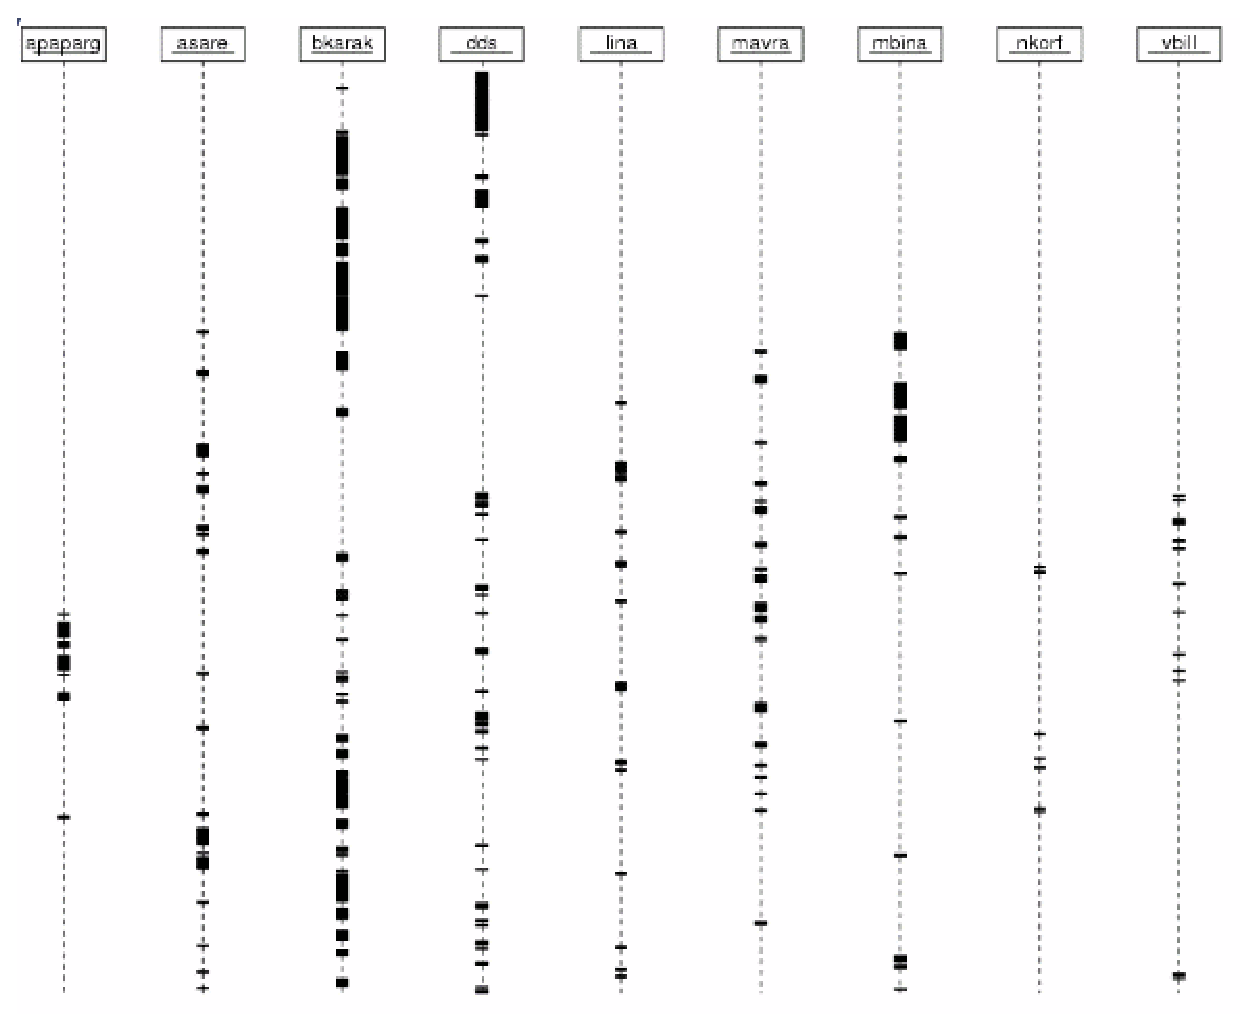
\includegraphics[scale=0.6]{cvs-log.eps}
\caption{Commit progress graph}
\label{fig:cvs-log}
\end{figure}

In Figure \ref{fig:cvs-log} we can see the {\sc CVS} commit commands that have been performed by
the Content Developers and Administrators. Each swimlane in the figure represents a committing
member of our system. Each horizontal line represents a single commit procedure. Content Administrators
are \textit{dds} (Diomidis Spinellis) and \textit{bkarak} (Vassilios Karakoidas). Initially we can see that only the two committed 
changes to the system. It was the period of development of the system. After the initial development, a few 
pioneer content developers started to use the system and commit {\sc XML} and bibliography data. In this period 
we also tested the system thoroughly and developed the finalized the presentation of the web site. After the end of
the test period all users became active and began to commit data in a parallel manner. This proves that we achieved 
one of our primary goals, make the web site procedure a multi-continuous development activity.

\section{Acknowledgments}
\label{sec:ack}

We would like to thank Prof. Manolis Skordalakis for his very perceptive comments during the compilation of this paper.
The authors would also like to thank Marianthi Theocharidou who reviewed early versions 
of this paper.

\bibliographystyle{unsrt}
\bibliography{declweb}

\end{document}